%%%%%%%% ICML 2023 EXAMPLE LATEX SUBMISSION FILE %%%%%%%%%%%%%%%%%

\documentclass[nohyperref]{article}


\usepackage{microtype}
\usepackage{graphicx}
\usepackage{subfigure}
\usepackage{booktabs} % for professional tables

% hyperref makes hyperlinks in the resulting PDF.
% If your build breaks (sometimes temporarily if a hyperlink spans a page)
% please comment out the following usepackage line and replace
% \usepackage{icml2023} with \usepackage[nohyperref]{icml2023} above.
\usepackage{hyperref}


% Attempt to make hyperref and algorithmic work together better:
\newcommand{\theHalgorithm}{\arabic{algorithm}}

% Use the following line for the initial blind version submitted for review:
\usepackage[accepted]{icml2023}

% If accepted, instead use the following line for the camera-ready submission:
% \usepackage[accepted]{icml2022}

% For theorems and such
\usepackage{amsmath}
\usepackage{amssymb}
\usepackage{mathtools}
\usepackage{amsthm}
\usepackage{array}
% if you use cleveref..
\usepackage[capitalize,noabbrev]{cleveref}

%%%%%%%%%%%%%%%%%%%%%%%%%%%%%%%%
% THEOREMS
%%%%%%%%%%%%%%%%%%%%%%%%%%%%%%%%
\theoremstyle{plain}
\newtheorem{theorem}{Theorem}[section]
\newtheorem{proposition}[theorem]{Proposition}
\newtheorem{lemma}[theorem]{Lemma}
\newtheorem{corollary}[theorem]{Corollary}
\theoremstyle{definition}
\newtheorem{definition}[theorem]{Definition}
\newtheorem{assumption}[theorem]{Assumption}
\theoremstyle{remark}
\newtheorem{remark}[theorem]{Remark}

% Todonotes is useful during development; simply uncomment the next line
%    and comment out the line below the next line to turn off comments
%\usepackage[disable,textsize=tiny]{todonotes}
\usepackage[textsize=tiny]{todonotes}


% The \icmltitle you define below is probably too long as a header.
% Therefore, a short form for the running title is supplied here:
\icmltitlerunning{RL Project report}

\newcommand{\dnl}{\mbox{}\par}
\newcommand{\mycomment}[1]{\textbf{Note:} \textit{#1}}
\newcommand{\cnote}[1]{\textsf{\color{blue} [#1]}}
%\newcommand{\cnote}[1]{}


\begin{document}

\twocolumn[
\icmltitle{Project Report: Default credit card}


\icmlsetsymbol{equal}{*}

\begin{icmlauthorlist}
\icmlauthor{Wahidullah Haidari(4033)}{}
\icmlauthor{Lkhanaajav Mijiddorj(4033)}{}
\end{icmlauthorlist}


\vskip 0.3in
]
\section{Abstract}
In this semester's 2nd Machine Learning project, our primary focus is on Supervised Learning - a cornerstone of machine learning that maps an input to an output based on example input-output pairs. The aim of our project is to develop a robust and accurate machine learning model that is capable of predicting the likelihood of credit card customers defaulting on their payments in the subsequent month. 

Credit default risk is a critical financial challenge faced by banks and other lending institutions. By accurately predicting default likelihood, these institutions can mitigate potential losses, adjust credit limits, and implement proactive strategies to manage risk more effectively. 

The success of the project will be measured by the accuracy of the model in predicting whether a customer will default on their payment in the following month. It is our hope that the results of this project will contribute to the development of more sophisticated, data-driven strategies for managing credit risk in the financial industry. 
\section{Projet Domain}
\subsection{Data}
In this project, we will use the "Default of Credit Card Clients" dataset from UCI, which comprises comprehensive data on credit card users in Taiwan from April 2005 to September 2005. This dataset includes 30,000 instances and 24 attributes, providing us with a substantial and diverse dataset for model training and validation. The attributes include demographic and financial information about each client such as gender, age, education, marital status, credit limit, repayment status, bill amount, and previous payments \cite{Yeh_2016}.

The aim of this project is to implement and compare the performance of four different supervised learning algorithms, namely logistic regression, decision tree, random forest, and neural networks, to predict whether a client will default on their credit card payment in the following month. By comparing the results of these algorithms, we can determine which performs best and can be used to make accurate predictions on the credit default dataset. \
\subsection{Learning method}
Quick definition of the each algorithm:

Logistic Regression: A statistical technique that functions the predictor variables to model the likelihood of a binary outcome.

Decision Trees: A tree-based algorithm that divides the data into more manageable subsets according to the predictor variables and builds a tree structure to predict the future.

Random Forest: A decision tree-based ensemble technique that combines different decision trees to produce predictions with higher accuracy.

Neural Networks: A machine learning algorithm that can be used to model intricate nonlinear relationships between the input and output variables and was inspired by the structure of the human brain.
\section{Hypotheses}
Hypothesis 1:
Younger people more likely to default than older people
We can compare the mean age of defaulters and non-defaulters to see which one of old and young is more likely go on default.

Hypothesis 2:
Random Forest algorithm will outperform Logistic Regression in predicting credit card defaults.

Hypothesis 3:
Sex, marriage, and education are less important independent variables for the dataset. 

Hypothesis 4:
We hypothesize that a neural network, due to its ability to model complex non-linear relationships, will outperform traditional machine learning models in predicting credit default risk. 
\section{Learning experiments}

Wahidullah Haidari implemented Logistic Regression and Decision Tree. Lkhanaajav Mijiddorj implemented Random Forest and Neural Networks. For all of these algorithms, we have divided the dataset into training, validating, and testing sets. For every algorithm, we have also plotted the learning curve for the number of the training set and its associated accuracy.

\subsection{Random Forest}
Our first algorithm, The Random Forest model, with 7 decision trees and a maximum depth of 3, demonstrated a steady rise in accuracy as the sample size was systematically increased. Specifically, accuracy progressed from 0.811 to 0.819. Ultimately, the model achieved a promising final accuracy of approximately 0.82. This suggests that the Random Forest model benefits from larger training data volumes, demonstrating improved generalization and predictive accuracy. However, the steady yet gradual increase in accuracy also indicates the possibility of reaching a higher point with further increases in sample size. This study underscores the value of considering sample size and model complexity (in terms of the number of trees and their maximum depth) in improving model performance in credit risk prediction tasks. Future investigations may aim to optimize these parameters further for enhanced predictive accuracy.

Random Forest Curve

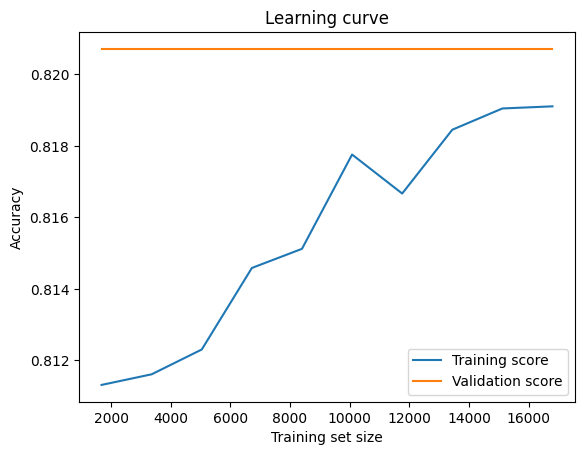
\includegraphics[scale=0.5]{Random Forest.png}

\subsection{Logistic Regression}

The second algorithm that we implemented is Logistic Regression. The model can predict the next month's default payment for 78 percent of the credit card users, according to the implementation's accuracy score of 0.78. By adjusting the training set size and graphing the accuracy scores on the training and test sets against the training set size, we can also create a learning curve. This learning curve assists in assessing the model's performance and determining if it is overfitting or underfitting. Overall, the approach can be helpful for forecasting credit card default payments because it is a quick and efficient technique to apply logistic regression to a binary classification problem.

Logistic Regression Curve

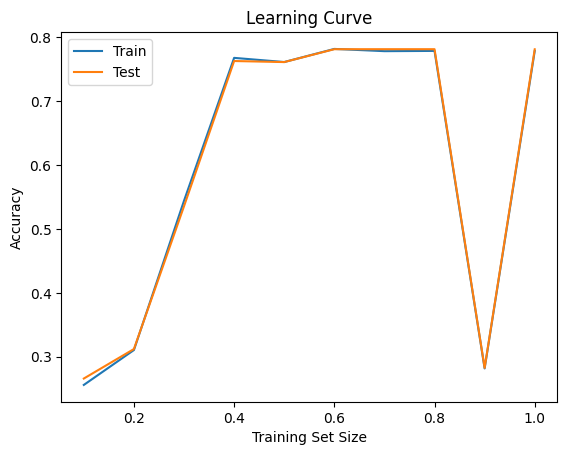
\includegraphics[scale=0.5]{Logistic Regression.png}


\subsection{Decision Tree}

In this instance, we used a decision tree classifier to forecast whether a specific person will default on a credit card. We used a validation set to adjust the maximum depth of the tree and avoid overfitting after training the model on the training set of the UCI credit card default dataset. To get a fair assessment of the model's performance, we lastly evaluated it on a testing set.

The results we obtained show that the decision tree algorithm achieved a validation accuracy of 0.842 and a testing accuracy of 0.832222. These accuracy scores indicate that the decision tree model is able to make accurate predictions on new, unseen data. 

 Decision Tree Learning Curve

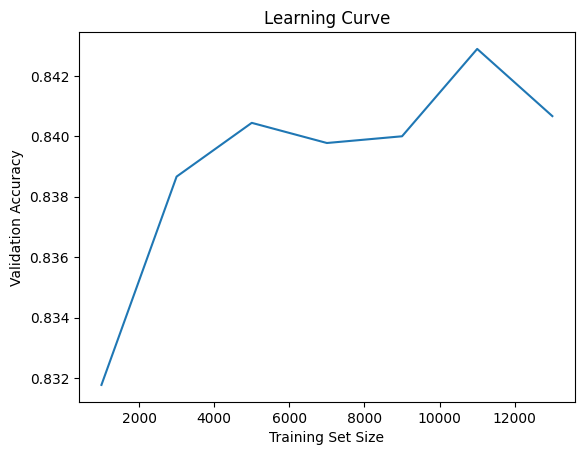
\includegraphics[scale=0.5]{Decision tree.png}

\subsection{Neural Networks}

For our final algorithm, we developed a neural network model to predict credit card defaults. The model consisted of one hidden layer and used the sigmoid activation function. To assess the model's performance, we employed k-fold cross-validation with k=5. This technique divided the training data into five subsets, training the model five times using each subset as the validation set while using the remaining subsets as the training set. By averaging the model's performance over multiple splits of the training data, we obtained a more reliable measure of its expected performance on unseen data.

During cross-validation, we calculated the mean squared error (MSE) as a measure of the model's loss. The average cross-validation MSE was approximately 0.356, with a standard deviation of 0.161. The variability in these results indicates that the model's performance is sensitive to the specific training set used. Therefore, further adjustments and regularization may be necessary to improve the model's consistency.

Subsequently, we trained a final model using the entire training set and evaluated its performance on a separate test set. The test set results showed a lower MSE compared to cross-validation, approximately 0.25. This discrepancy suggests that the model may be overfitting the training data to some extent, even with cross-validation. Future work can focus on addressing overfitting by exploring techniques such as adding regularization terms to the loss function or incorporating dropout or batch normalization layers into the model architecture.

\section{Analysis and Explanations}

\subsection{First Hypothesis:}
The analysis of the dataset suggests that there is a slight difference in the default rates between younger and older people. The default rate for younger people (age less than 30) is approximately 22.84 percent, while the default rate for older people (age more than equal to  30) is slightly lower at around 21.78 percent. To determine the significance of this difference, a statistical test (t-test) was performed, resulting in a p-value of 0.0383. With a significance level of 0.05, this p-value indicates that there is a statistically significant difference in default rates between the two age groups. However, it is important to note that the observed difference, although statistically significant, is relatively small. As a result for this hypothesis, we can confirm that younger people more likely to go on default but it is not significant factor for going on default.

\subsection{Second Hypothesis:}
Despite its slower training process and increased model complexity, the Random Forest model outperformed logistic regression in terms of accuracy thanks to its ability to capture complex patterns, nonlinear relationships, and feature interactions. By combining multiple decision trees, the Random Forest model demonstrated greater robustness against over-fitting and proved to be more stable with respect to changes in the dataset. We have tried different hyperparameters for the number of trees and max depth and ended up with the number of trees as 7 and the max depth as 3. The accuracy score of the model was 0.81, while the logistic regression had an accuracy score of 0.78. Therefore, the hypothesis that the Random Forest model would outperform the logistic regression was confirmed.

\subsection{Third Hypothesis:}
When we dropped the sex, education, and marriage columns from the UCI credit card default dataset and trained the decision tree model on the remaining features, we obtained a validation accuracy of 0.842222 and a testing accuracy of 0.832222. These results indicate that the decision tree model could still achieve relatively high accuracy scores despite removing several independent variables. This suggests that the remaining features in the dataset may be more important predictors of credit card default than the dropped variables, which confirms our third hypothesis.

However, it's important to note that these results are specific to the UCI credit card default dataset and may not generalize to other datasets or real-world scenarios. Overall, the decision tree algorithm is a useful tool for predicting credit card default and has shown promising results on this particular dataset.

\subsection{Fourth Hypothesis:}
For the last hypothesis, we proposed the hypothesis that a neural network, with its inherent capacity to model complex non-linear relationships, would outperform traditional machine learning models in predicting credit default risk. The cross-validation yielded a mean squared error of approximately 0.356 with a standard deviation of 0.161, while the test set resulted in a lower mean squared error of 0.25. These promising results suggest that our neural network can effectively predict credit default risk. However, to definitively confirm our hypothesis.Furthermore, while our results highlight the potential of neural networks to outperform simpler models, they also underline the complexities involved, including the risk of over-fitting and the need for careful tuning of model parameters. Despite these challenges, our study provides a strong basis for further exploration of neural networks in credit default risk prediction.

\section{Related Work / Literature Review}
Credit Card Default Prediction Using Artificial Neural Networks" by Malik Mubasher Hassan and Tabasum Mirza is an article that explores the use of artificial neural networks (ANNs) for predicting credit card default. The UCI default on credit card dataset is used by the authors to train and evaluate their ANN model. Additionally, they contrast their findings with those of decision trees and logistic regression. The article analyzes the accuracy, sensitivity, specificity, and area under the curve (AUC) performance of the ANN model. The authors come to the conclusion that the ANN model, which achieved an AUC of 0.77, beats logistic regression and decision trees in predicting credit card default. In addition to highlighting the significance of model selection in credit risk prediction, the article offers insights into the potential of ANNs for credit risk assessment\cite{article}.

One related work to the project is a research paper focusing on the performance evaluation of credit card default prediction and the use of logistic regression, decision tree (rpart), and random forest algorithms. The paper addresses the escalating credit card default rate faced by banks and emphasizes the importance of data analytics in managing credit risks. Through their evaluation, they found that random forest exhibited the highest accuracy and area under the curve in predicting credit default. This research demonstrates the effectiveness of random forest in assessing credit risk for credit card customers, achieving an accuracy of 82 percent and an Area under Curve of 77 percent. The findings contribute valuable insights into the application of different algorithms for credit card default prediction, aiding banks in managing credit risk effectively \cite{8776802}.


\section{Summary and future work}
Summary:
In this project, Wahidullah Haidari and Lkhanaajav Mijiddorj, we have focused on developing a robust and accurate machine learning model to predict the likelihood of credit card customers defaulting on their payments in the next month. We have used the "Default of Credit Card Clients" dataset from UCI, which included demographic and financial information about credit card users in Taiwan. The project compared the performance of four different supervised learning algorithms: logistic regression, decision trees, random forest, and neural networks.

Wahidullah Haidari implemented logistic regression and decision tree algorithms, while Lkhanaajav Mijiddorj implemented random forest and neural networks. Each algorithm was evaluated using training, validating, and testing sets, and their learning curves were plotted to analyze the accuracy of predictions.

The results showed that the random forest model achieved an accuracy of approximately 0.82, indicating its effectiveness in predicting credit card defaults. Logistic regression obtained an accuracy score of 0.78, while the decision tree algorithm achieved validation and testing accuracy of 0.842 and 0.832222, respectively. The neural network model had a mean squared error of approximately 0.356 during cross-validation and 0.25 on the test set.

Future Work:
For future work, several aspects can be explored to further enhance the project:

1. Feature Engineering: Consider additional feature engineering techniques to extract more relevant information from the dataset, potentially improving the models' predictive performance.

2. Hyper-parameter Tuning: Explore different hyper-parameter configurations for each algorithm to optimize their performance. Especially, we should try different parameters for the random forest since it showed promising result and according to the one of the related work, it shows that random forest could be the best one for this case.

3. Real-time Prediction: Implement the best-performing model in a real-time environment, where it can make predictions on new credit card transactions and provide timely risk assessment for lending institutions.

By addressing these aspects, the project can provide further improvement into credit card default prediction and contribute to the development of more accurate and reliable strategies for managing credit risk in the financial industries and banks. Also, we can make conclusion of which of the algorithmn is suited for this case. 

\bibliographystyle{plainnat}
\bibliography{refs.bib}
\end{document}


